% 实验二过程与结果
\subsection{实验过程与结果}

\subsubsection{实验设置}
构造 3 组 $\Lambda$-集合，每组包含 256 个明文，在矩阵坐标 $(1,0)$ 处遍历。分别测试 3 轮、4 轮以及无 MixColumns 情况下的异或和。
我们选取的明文如下：
% Plain 0
\[
P_0 = \begin{bmatrix}
16 & 34 & 52 & 70 \\
* & 106 & 124 & 142 \\
145 & 163 & 181 & 199 \\
217 & 235 & 253 & 15
\end{bmatrix}
\]

% Plain 1
\[
P_1 = \begin{bmatrix}
1 & 19 & 37 & 55 \\
* & 91 & 109 & 127 \\
128 & 146 & 164 & 182 \\
200 & 218 & 236 & 254
\end{bmatrix}
\]
% Plain 2
\[
P_2 = \begin{bmatrix}
255 & 238 & 221 & 204 \\
* & 170 & 153 & 136 \\
119 & 102 & 85 & 68 \\
51 & 34 & 17 & 0
\end{bmatrix}
\]
我们选择的密钥如下：\\
\[
\text{key = 0xabf266f7a189b08e5db4a56ea585ae0f}
\]
\subsubsection{结果记录}
保持MC变换,代码运行结果如下
\begin{figure}[H]
    \centering
    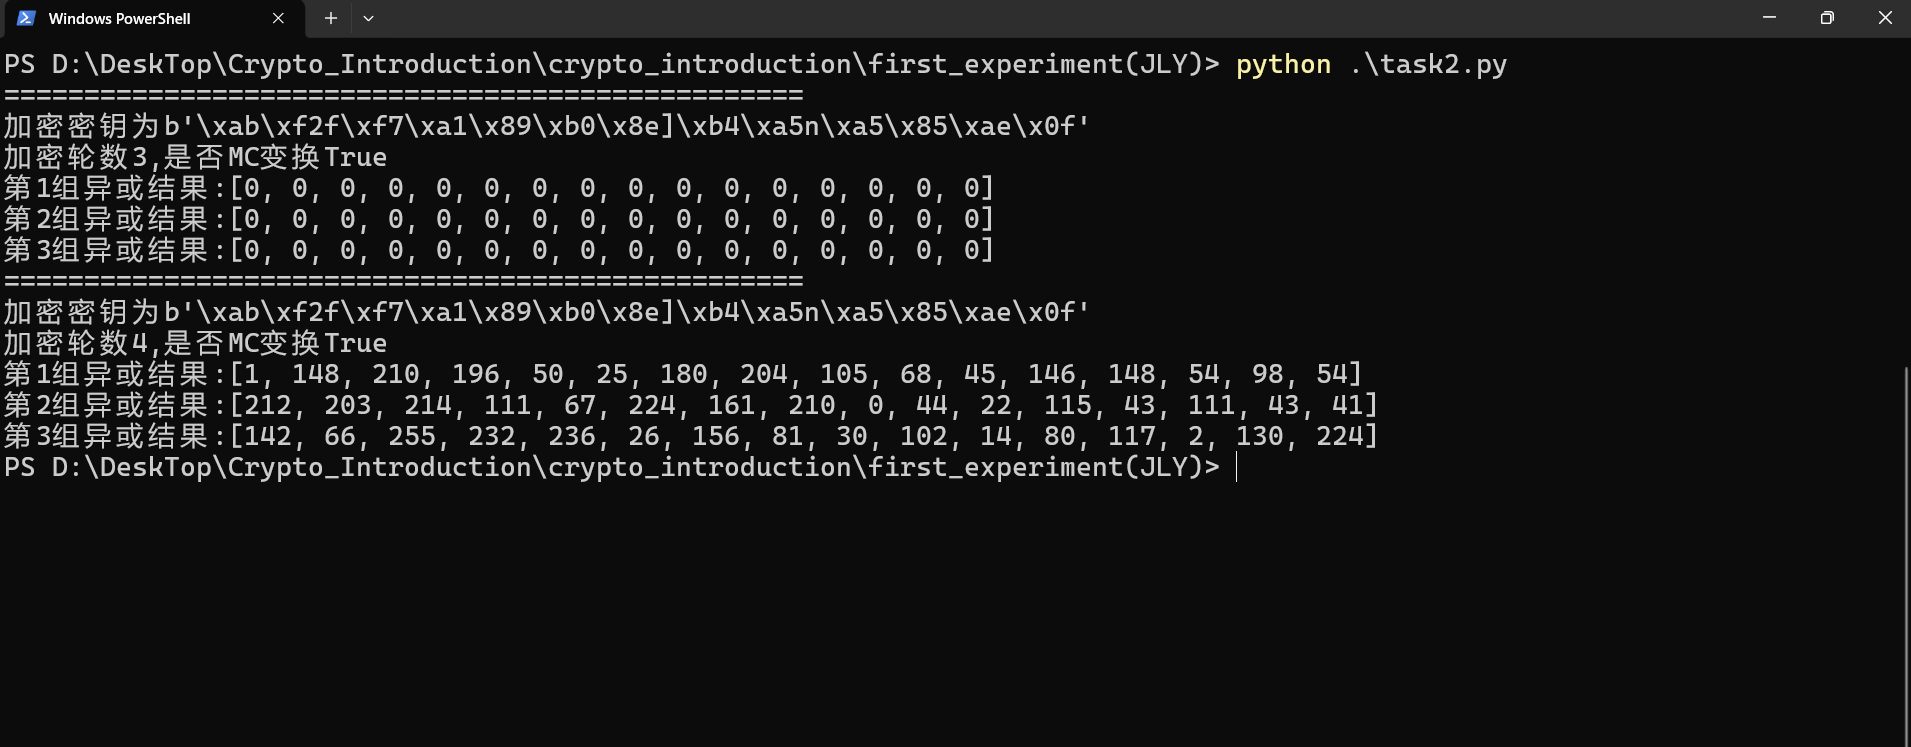
\includegraphics[width = 1\textwidth]{figure/task2_run3_4.png}
    \caption{3轮和4轮AES加密、结果异或(保持MC变换)}
\end{figure}
可以看到当AES加密轮数为3组时,这3个实验组变动位遍历0~255的每组总计256种密文加密后的异或结果均为0,但当AES加密轮数变为4轮后异或结果就变得各不相同。\\

删去MC变换,代码运行结果如下

\begin{figure}[H]
    \centering
    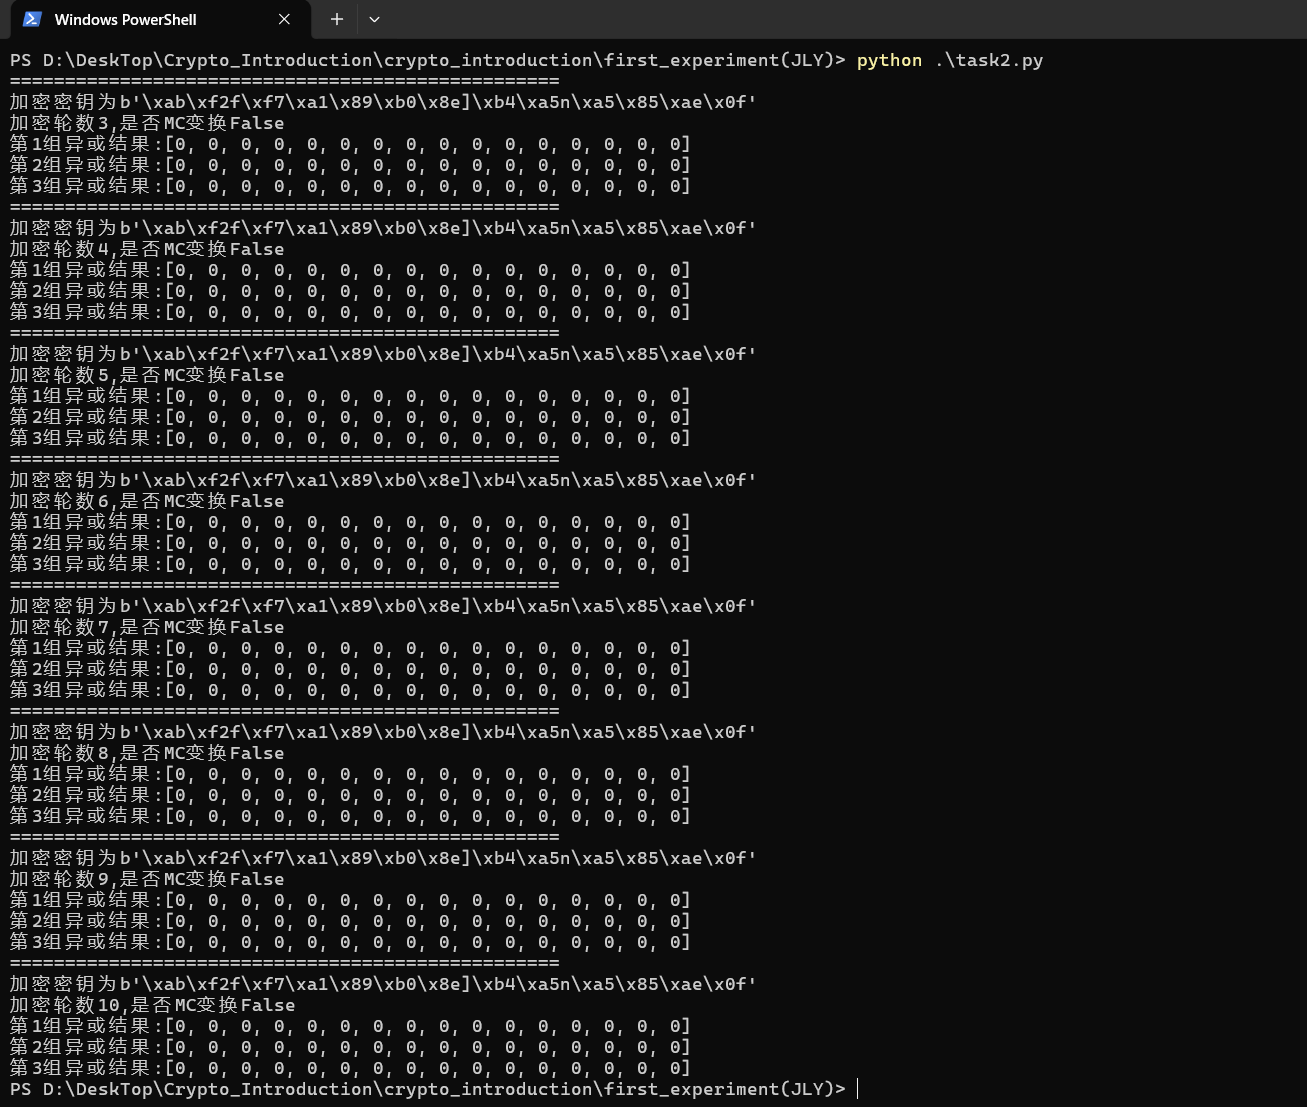
\includegraphics[width = 0.8\textwidth]{figure/task2_10rounds.png}
    \caption{10轮AES加密、结果异或(删除MC变换)}
\end{figure}
当删除MC变换时,相同数据和代码,即使加密10轮,各组的异或结果也都是0

% 检查发现你的代码跟pdf中内容不一致,用我的代码，使用pdf中数据,结果放的截图
%=========================================================
% 根据实验运行结果，记录如下表：
% (三组明文得到的结果都是一样的，对于4轮的情况，由于数据太长，只写了第一个)
% \begin{table}[h]
%     \centering
%     \begin{tabular}{@{}cccc@{}}
%         \toprule
%         实验组别 & 轮数 & 包含 MixColumns & 异或结果 (XOR Sum) \\ \midrule
%         1        & 3    & 是               & $[0, 0, 0]$ (平衡)         \\
%         2        & 4    & 是               &$[213218948687531644049869954314427593478, ...]$ (不平衡) \\
%         3        & 4-31 & \textbf{否}      & $[0, 0, 0]$ (始终平衡)     \\ \bottomrule
%     \end{tabular}
%     \caption{不同配置下的 AES 异或实验结果}
% \end{table}
%=========================================================